\documentclass[11pt]{amsart}
\usepackage{amsmath,amsthm,amsfonts,amssymb,enumerate}
\usepackage[normalem]{ulem}
\usepackage{ dsfont }
\usepackage{geometry}
\usepackage{graphicx}
\usepackage{float}


\title{Convex and Nonsmooth Optimization:\\HW 3}
\author{Terrence Alsup}
\date{February 25, 2020}

\begin{document}
\maketitle
\begin{enumerate}
%%%%%%%%%%%%%%%%%%%%%%%%%%%%%%%%%%%%%%%%%%%
\item \begin{enumerate}
\item The Lagrangian is
\[
L(x, \nu) = \frac{1}{2}x^TQx + \nu^T(Ax - b)
\]
with $\nu \in \mathbb{R}^m$.





\item Taking the gradient with respect to the variable $x$ gives
\[
\nabla_x L(x, \nu) = Qx + A^T\nu
\]
Note that for the derivatives in this homework I used the Matrix Cookbook \texttt{https://www.math.uwaterloo.ca/${\sim}$hwolkowi/matrixcookbook.pdf}.  Setting the gradient to zero gives
\[
Qx + A^T\nu = 0
\]
Since $Q$ is (strictly) positive definite, it is invertible and we can write $x = -Q^{-1}A^T\nu$.  Plugging this into the Lagrangian gives the Lagrange dual function
\begin{align*}
g(\nu) = \inf_x L(x, \nu) &= L(-Q^{-1}A^T\nu, \nu)\\
&= \frac{1}{2}(Q^{-1}A^T\nu)^TQ(Q^{-1}A^T\nu) + \nu^T(-AQ^{-1}A^T\nu - b)\\
&= \frac{1}{2}\nu^T A Q^{-1}QQ^{-1}A^T \nu - \nu^TAQ^{-1}A^T\nu - \nu^T b\\
&= -\frac{1}{2} \nu^T  AQ^{-1}A^T \nu - b^T \nu
\end{align*}




%\item Taking the gradient with respect to the variable $x$ gives
%\[
%\nabla_x L(x, \nu) = Qx + A^T\nu
%\]
%and similarly for $\nu$
%\[
%\nabla_{\nu} L(x, \nu) = Ax - b
%\]
%Note that for these derivatives I used the Matrix Cookbook \texttt{https://www.math.uwaterloo.ca/${\sim}$hwolkowi/matrixcookbook.pdf}.  Setting the gradient to zero gives
%\[
%\begin{cases}
%Qx + A^T\nu = 0\\
%Ax - b = 0
%\end{cases}
%\]
%Since $Q$ is (strictly) positive definite, it is invertible and we can write $x = -Q^{-1}A^T\nu$.  Plugging this into the second equation gives
%\[
%-AQ^{-1}A^T\nu - b = 0
%\]
%Since $Q$ is symmetric and positive definite its inverse is also symmetric and positive definite and therefore has a symmetric square root $Q^{-1/2} = (Q^{-1/2})^T$ with $Q^{-1/2}Q^{-1/2} = Q^{-1}$.  Thus, we can write
%\[
%AQ^{-1}A^T = AQ^{-1/2}Q^{-1/2}A^T = (Q^{-1/2}A^T)^T(Q^{-1/2}A^T)
%\]
%which is of the form $B^TB$.  Since $A$ is of full rank we know that $B^TB = AQ^{-1}A^T$ is invertible.  Hence we can solve
%\[
%\nu = -(AQ^{-1}A^T)^{-1}b
%\]
%and therefore,
%\[
%x = Q^{-1}A^T(AQ^{-1}A^T)^{-1}b
%\]
%Plugging in these values for $x,\nu$ give
%\begin{align*}
%p^* = L(x, \nu) = &\frac{1}{2} (Q^{-1}A^T(AQ^{-1}A^T)^{-1}b)^TQQ^{-1}A^T(AQ^{-1}A^T)^{-1}b \\
%&- ((AQ^{-1}A^T)^{-1}b)^T(AQ^{-1}A^T(AQ^{-1}A^T)^{-1}b - b)
%\end{align*}
%Simplifying gives
%\[
%p^* = 
%\]








\item Setting the gradient of the dual function to zero gives
\[
\nabla_{\nu}g(\nu) = -AQ^{-1}A^T \nu - b = 0
\]
and therefore the maximizer of the dual function is 
\[
\nu^* = -(AQ^{-1}A^T)^{-1}b
\]
and plugging this in gives the dual optimal value
\begin{align*}
d^* &= g(\nu^*)\\
&= -\frac{1}{2} (\nu^*)^T  AQ^{-1}A^T \nu^* - b^T \nu^*\\
&= -\frac{1}{2} ((AQ^{-1}A^T)^{-1}b)^T AQ^{-1}A^T (AQ^{-1}A^T)^{-1}b + b^T(AQ^{-1}A^T)^{-1}b\\
&= -\frac{1}{2} ((AQ^{-1}A^T)^{-1}b)^Tb + b^T(AQ^{-1}A^T)^{-1}b\\
&= -\frac{1}{2} b^T (AQ^{-1}A^T)^{-1}b + b^T(AQ^{-1}A^T)^{-1}b\\
&= \frac{1}{2} b^T (AQ^{-1}A^T)^{-1}b
\end{align*}
Note that the second to last line follows from the fact that since $AQ^{-1}A^T$ is invertible and symmetric then its inverse is symmetric.






\item To find the minimizer $\hat{x}$ for $L(x,\nu^*)$ we again set the gradient to zero.
\[
\nabla_x L(x,\nu^*) = Qx + A^T \nu^* = 0
\]
Thus,
\begin{align*}
\hat{x} &= -Q^{-1}A^T\nu^*\\
&= Q^{-1}A^T(AQ^{-1}A^T)^{-1}b
\end{align*}



\item We check primal feasibility by looking at whether $A\hat{x} = b$ and compute directly
\begin{align*}
A\hat{x}&= AQ^{-1}A^T(AQ^{-1}A^T)^{-1}b = b
\end{align*}
since the inverse cancels $AQ^{-1}A^T$.  Thus, $\hat{x}$ is feasible for the primal problem.






\item The primal value $f_0(\hat{x})$ is
\begin{align*}
f_0(\hat{x}) &= \frac{1}{2}\hat{x}^TQ\hat{x}\\
&= \frac{1}{2} (Q^{-1}A^T(AQ^{-1}A^T)^{-1}b)^TQQ^{-1}A^T(AQ^{-1}A^T)^{-1}b\\
&= \frac{1}{2} b^T (AQ^{-1}A^T)^{-1}AQ^{-1}QQ^{-1}A^T(AQ^{-1}A^T)^{-1}b\\
&= \frac{1}{2} b^T (AQ^{-1}A^T)^{-1} AQ^{-1}A^T(AQ^{-1}A^T)^{-1}b\\
&= \frac{1}{2}b^T (AQ^{-1}A^T)^{-1}b
\end{align*}


\item We conclude that there is no duality gap since $p^* \ge d^* = f_0(\hat{x}) \ge p^*$ meaning $d^* = p^*$.

\end{enumerate}

%%%%%%%%%%%%%%%%%%%%%%%%%%%%%%%%%%%%%%%%%%%


\vspace{0.5in}


%%%%%%%%%%%%%%%%%%%%%%%%%%%%%%%%%%%%%%%%%%%
\item \begin{enumerate}

\item The feasible set is $\{x\in \mathbb{R} : (x-2)(x-4) \le 0\}$ for $(x-2)(x-4) \le 0$ we must have that $x-2$ and $x-4$ have opposite signs (or one is zero).  Thus, the feasible set is just the interval $[2,4]$.  The optimal value is $5$ and occurs at $x = 2$.



\item For this problem the Lagrangian is
\[
L(x,\lambda) = x^2 + 1 + \lambda(x-2)(x-4)
\]
This is quadratic with positive coefficient when $\lambda > -1$.  If $\lambda \le -1$ then we either have a quadratic term with negative coefficient or a linear term with negative coefficient (in the case $\lambda = -1$).  In either of these cases the Lagrangian is unbounded below in $x$.  We can rewrite
\[
L(x,\lambda) = (1 + \lambda)x^2 - 6 \lambda x + (8\lambda  + 1)
\]
when $\lambda > -1$ the minimizer is $x = \frac{3\lambda}{1 + \lambda}$.  Plugging this into the Lagrangian gives
\[
L(x(\nu),\nu) = \frac{9\lambda^2}{1 + \lambda} - \frac{18\lambda^2}{1 + \lambda} + 8\lambda +1 
\]
Thus, the Lagrange dual function is
\[
g(\lambda) = \begin{cases} -\frac{9\lambda^2}{1 + \lambda} + 8\lambda + 1, & \lambda > -1\\
-\infty, & \lambda \le -1
\end{cases}
\]
The first plot below shows the objective function $f_0(x) = x^2 + 1$ over the feasible set $[2,4]$ with the Lagrangian for several $\lambda$.  The second plot shows the Lagrange dual function.

\begin{figure}[H]
\centering
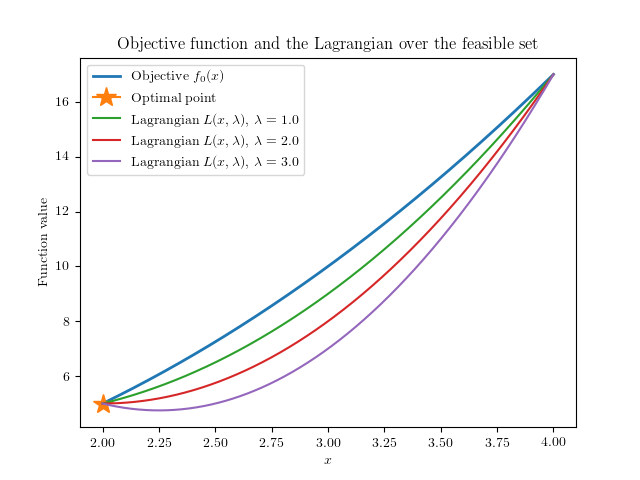
\includegraphics[width=5in]{fig1.png}
\caption{The objective function over the feasible set with the Lagrangian evaluated at $\lambda = 1,2,3$.}
\end{figure}

\begin{figure}[H]
\centering
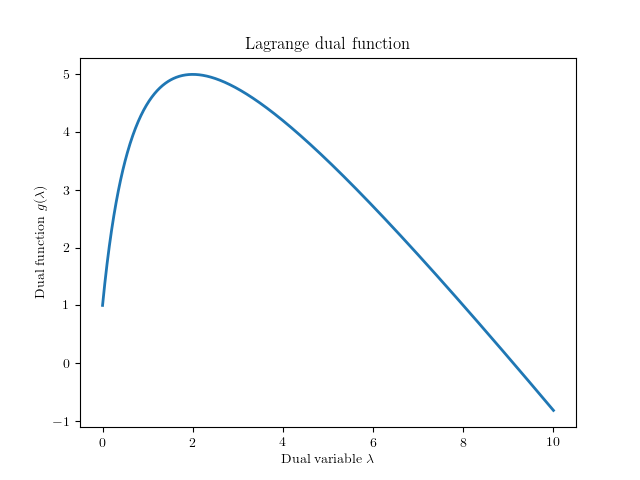
\includegraphics[width=5in]{fig2.png}
\caption{The Lagrange dual function $g(\lambda)$ vs. $\lambda$.}
\end{figure}





\item  The dual problem is
\[
\underset{\lambda \ge 0}{\mathrm{maximize}} -\frac{9\lambda^2}{1 + \lambda} + 8\lambda + 1
\]
To see that this is concave we compute the second derivative when $\lambda \ge 0$.
\[
\frac{d}{d\lambda}g(\lambda) = -\frac{9\lambda^2 + 18\lambda}{(1 + \lambda)^2} + 8
\]
and
\[
\frac{d^2}{d\lambda^2}g(\lambda) = -\frac{18}{(1 + \lambda)^3} < 0
\]
Since the second derivative is always negative when $\lambda \ge 0$ we know that this is a concave maximization problem.  To find the dual optimal solution $\lambda^*$ we set the derivative to zero and get
\[
\frac{9\lambda^2 + 18\lambda}{(1 + \lambda)^2} = 8
\]
Simplifying gives the following quadratic equation for $\lambda$.
\[
\lambda^2 + 2\lambda - 8 = (\lambda + 4)(\lambda - 2) = 0
\]
Since we must have $\lambda^* \ge 0$ we know that $\lambda^* = 2$ is the optimal dual solution and
\[
d^* = g(\lambda^*) = 5
\]
is the optimal dual value.  Indeed strong duality holds since $d^* = p^* = 5$.




\item The constraint can be written as
\[
x^2 - 6x + (8-u) \le 0
\]
Since this is a quadratic equation with positive coefficient, the feasible set is the interval between the (real) roots of the equation.  Thus, we solve to find that the roots are
\[
x = 3 \pm \sqrt{1 + u}
\]
Note that if $u < -1$ then there are no real roots and hence the feasible set is empty.  Since the objective is a minimization over $x^2 + 1$ we see that we must take $x$ to be the smaller root.  Hence the optimal solution is
\[
x^* = 3 - \sqrt{1 + u}
\]
and
\[
p*(u) = u - 6\sqrt{u + 1} + 11
\]
The figure below shows the plot of $p^*(u)$ for $u \in [-1, 10]$.  Taking the derivative at $u = 0$ gives
\[
\frac{d}{du}p^*(u) = 1 - \frac{3}{u + 1} \implies \frac{d}{du}p^*(0) = -2
\]
which is the same as $-\lambda^*$.
\begin{figure}[H]
\centering
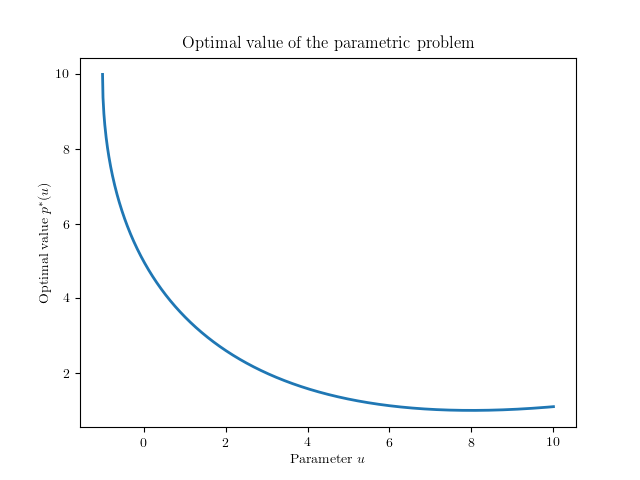
\includegraphics[width=5in]{fig3.png}
\caption{The optimal value $p^*(u)$ vs. $u$.}
\end{figure}

\end{enumerate}

%%%%%%%%%%%%%%%%%%%%%%%%%%%%%%%%%%%%%%%%%%%

\vspace{0.5in}


%%%%%%%%%%%%%%%%%%%%%%%%%%%%%%%%%%%%%%%%%%%

\item \begin{enumerate}
\item To see that this is a convex optimization problem we show that $f_0(x,y) = e^{-x}$ and $f_1(x,y) = x^2/y$ are convex.  In particular, we will show that their Hessians are positive semi-definite.  We easily compute
\[
\nabla \nabla^T f_0(x,y) = \begin{bmatrix} e^{-x} & 0\\0&0  \end{bmatrix}
\]
which is diagonal so its eigenvalues are $e^{-x}$ and $0$.  Thus, the objective is convex.  For the constraint we compute
\[
\nabla \nabla^T f_1(x,y) = \begin{bmatrix}
2y^{-1} & -2xy^{-2}\\
-2xy^{-2} & 2x^2y^{-2}
\end{bmatrix}
\]
We will use the facts that the sum of the eigenvalues is the trace and the determinant of the matrix is the product of the eigenvalues.  The determinant is 0, however, so we know at least one eigenvalue is zero.  The other eigenvalue is just the trace which is
\[
2y^{-1} + 2x^2y^{-2} > 0
\]
Since all eigenvalues are non-negative, the Hessian is positive semi-definite.  Therefore, this is indeed a convex optimization problem.\\
\\
Since $x^2,y > 0$, we must have the $x = 0$ to satisfy the constraint.  Thus, we trivially have that the optimal value is $f_0(x^*) = f_0(0) = 1$, where $x^* = 0$.





\item The Lagrangian for this problem is given by
\[
L(x,y,\lambda) = e^{-x} + \lambda x^2 y^{-1}
\]
If $\lambda \ge 0$ is fixed, then the infimum is just zero because we can take $y = x^3$ and send $x \to \infty$ for instance.  Thus, the Lagrange dual function is simply
\[
g(\lambda) = \begin{cases}
0, & \lambda \ge 0\\
-\infty, & \lambda < 0
\end{cases}
\]
Therefore, the dual problem is
\[
\underset{\lambda \ge 0}{\mathrm{maximize}}\ 0
\]
meaning that the optimal value $d^* = 0$ and the optimal duality gap is $p^* - d^* = 1$.




\item For this problem Slater's condition does not hold because $x^2 y^{-1} \ge 0$ for all $(x,y) \in \mathcal{D}$.  Moreover, the interior is empty anyways.


\item For the perturbed problem we have no solution when $u < 0$.  When $u > 0$ we must take $x^2 \le uy$.  To make $e^{-x}$ we must take $x$ as large as possible and hence the optimal value for $x$ is $\sqrt{uy}$.  Taking $y \to \infty$ means $x\to \infty$ and the optimal value is $p^*(u) = 0$.  Thus,
\[
p^*(u) = \begin{cases}
\infty, & u < 0\\
1, & u = 0\\
0 & u > 0
\end{cases}
\]
We see now that the global sensitivity inequality does not hold because we have for $u > 0$
\[
p^*(u) = 0 < p^*(0) - \lambda^*u = 1 -\lambda^* u
\]
whenever $u$ is sufficiently small.
\end{enumerate}


%%%%%%%%%%%%%%%%%%%%%%%%%%%%%%%%%%%%%%%%%%%




\vspace{0.5in}



%%%%%%%%%%%%%%%%%%%%%%%%%%%%%%%%%%%%%%%%%%%
\item First we note that the domain of the problem $\mathcal{D}$ is convex because it is the intersection of convex sets.  Suppose that $(u_1,v_1,t_1),\ (u_2,v_2,t_2) \in \mathcal{A}$ and let $\theta \in [0,1]$.  By definition, there exist points $x_1,x_2 \in \mathcal{D}$ so that $f_i(x_j) \le u_j$, $h_i(x_j) = v_j$ and $f_0(x_j) \le t_j$ for $j=1,2$.  By convexity of $\mathcal{D}$ we know that $\theta x_1 + (1-\theta)x_2 = x \in \mathcal{D}$.  We have that
\[
f_i(x) = f_i(\theta x_1 + (1-\theta)x_2) \le \theta f_i(x_1) + (1-\theta)f_i(x_2) \le \theta u_1 + (1-\theta)u_2
\]
for each $i=1,\ldots,m$ since $f_i$ is convex.  Moreover, since $h_i(y)$ is affine we can write $h_i(y) = A_iy + b_i$ and
\[
h_i(x) = A_ix + b_i = \theta (A_i x_1 + b_i) + (1-\theta)(A_i x_2 + b_i) = \theta v_1 + (1-\theta)v_2
\]
Finally, we have 
\[
f_0(x) \le \theta f_0(x_1) + (1-\theta)f_0(x_2) \le \theta t_1 + (1-\theta)t_2
\]
Thus, 
\[
 \begin{bmatrix}
\theta u_1 + (1-\theta)u_2\\
\theta v_1 + (1-\theta)v_2\\
\theta t_1 + (1-\theta)t_2
\end{bmatrix} \in \mathcal{A}
\]
and $\mathcal{A}$ is convex.
%%%%%%%%%%%%%%%%%%%%%%%%%%%%%%%%%%%%%%%%%%%


\vspace{0.5in}



%%%%%%%%%%%%%%%%%%%%%%%%%%%%%%%%%%%%%%%%%%%
\item \begin{enumerate}


\item Consider that for the Boolean LP, if $x_i \in \{0,1\}$, then also $0 \le x_i \le 1$ so if the constrains of the Boolean LP are satisfied then so are the constraints for the relaxed LP.  Thus, the feasible set for the Boolean LP is a subset of the feasible set for the relaxed LP.  Since we are minimizing over a larger set, we know that a solution to the relaxed LP will be a lower bound to the solution of the Boolean LP.  Moreover, if the LP relaxtion is infeasible then there is also no point that will satisfy the Boolean LP and hence the Boolean LP is also infeasible.


\item If the LP relaxation has a solution with $x_i \in \{0,1\}$, then we automatically know that this is also the solution to the Boolean LP.  This is because it is a feasible point for the Boolean LP and achieves the lower bound imposed by the LP relaxation. 






\end{enumerate}







%%%%%%%%%%%%%%%%%%%%%%%%%%%%%%%%%%%%%%%%%%%
\end{enumerate}





\end{document}